\documentclass[12pt,twoside, a4paper]{article}
\usepackage[utf8]{inputenc}
\usepackage[brazil]{babel}
\usepackage[margin = 0.5in]{geometry}
\usepackage{amsmath}
\usepackage{amsthm}
\usepackage{amssymb}
\usepackage{amsthm}
\usepackage{setspace}
\usepackage[americanvoltages,fulldiodes,siunitx]{circuitikz}
\usepackage{lipsum}
\usepackage{pgfplots}
\usepackage{ifthen}
\usepackage{adjustbox}
\usepackage[section]{placeins}
\usepackage{hyperref}
\usepackage{graphicx}
\usepackage{amsmath}
\usepackage{amsthm}
\usepackage{amssymb}
\usepackage{amsthm}
\usepackage{setspace}
\usepackage[americanvoltages,fulldiodes,siunitx]{circuitikz}
\usepackage{lipsum}
\usepackage{pgfplots}
\usepackage{ifthen}
\usepackage{adjustbox}
\usepackage[section]{placeins}
\usepackage{hyperref}
\usepackage{graphicx}
\usepackage{adjustbox}
\usepackage{indentfirst}
\usepackage{float}
\usepackage{pythonhighlight}


\pgfplotsset{compat=newest}
\graphicspath{ {./images/} }
%  #1 color - optional #2 x_0 #3 y_0 #4 x_f #5 y_f #6 name - optional  #7 true if adding lines to axis
\newcommand{\drawvector} [9] [color=cyan] {
\draw[line width=1.5pt,#1,-stealth](axis cs: #2, #3)--(axis cs: #4, #5) node[anchor=south west]{$#6$};
\ifthenelse{\equal{#7}{true}}{
\draw[line width=1pt,#1, dashed](axis cs: #4, #5)--(axis cs: #4, 0) node[anchor= north west]{$#8$};
\draw[line width=1pt,#1, dashed](axis cs: #4, #5)--(axis cs: 0, #5) node[anchor=south east]{$#9$};
}
{}
}
\newcommand\deriv[2]{\frac{\mathrm d #1}{\mathrm d #2}}
\title{Primeiro Relatório de Lab de Eletronica 1}
\author{Henrique da Silva \\ henrique.pedro@ufpe.br}
\date{\today}
\pgfplotsset{width = 10cm, compat = 1.9}
\begin{document}
\maketitle
\pagenumbering{gobble}
% \newpage
%pagenumbering{roman}
\tableofcontents
\newpage



\input{Sections/intro}

\section{Análise preliminar}

Utilizarei a biblioteca \emph{sympy} do \emph{Python} para fazer a análise simbólica e numérica do circuito antes de montá-lo fisicamente.

Após terminar as análises compararei os resultados obtidos nas análises numéricas e em laboratório para verificar sua coerência.

\subsection{O circuito}

\begin{figure}[h]
    \centering
    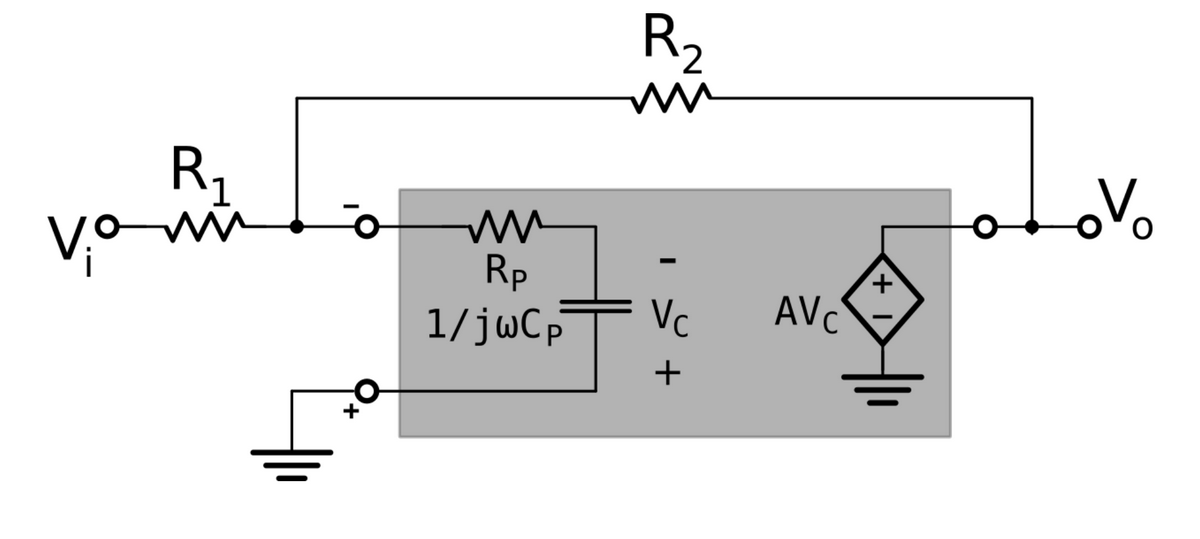
\includegraphics[width=1\columnwidth]{images/circuito.png}
    \caption{Circuito com amp op em configuração inversora.}
\end{figure}


\newpage
\subsection{Análise simbólica}


Podemos realizar a análise do circuito utilizando análise nodal.


\begin{equation}
    \begin{aligned}
        0       & = \frac{V_{a}}{R_{p} + \frac{1}{C_{p} j w}} + \frac{V_{a} - V_{o}}{R_{2}} + \frac{V_{a} - V_{i}}{R_{1}} \\
        - V_{c} & = \frac{V_{a}}{C_{p} j w \left(R_{p} + \frac{1}{C_{p} j w}\right)}                                      \\
        V_{o}   & = A V_{c}
    \end{aligned}
\end{equation}


Resolvendo as equações para $V_o$ obtemos que $V_o$ é dado por:


\begin{equation}
    - \frac{A R_{2} V_{i}}{A R_{1} + C_{p} R_{1} R_{2} j w + C_{p} R_{1} R_{p} j w + C_{p} R_{2} R_{p} j w
        + R_{1} + R_{2}}
\end{equation}


Aqui fazemos a seguinte simplificação $R_p >> R_1$ , $R_p >> R_2$, e $A >> 1$:


\begin{equation}
    V_o = - \frac{A R_{2} V_{i}}{A R_{1} + C_{p} R_{p} j w \left(R_{1} + R_{2}\right)}
\end{equation}


Com esta simplificação fazemos $\frac{V_o}{V_i}$ para obter a função transferência $H\left(jw\right)$:


\begin{equation}
    H\left(jw\right) = - \frac{A R_{2}}{A R_{1} + C_{p} R_{p} j w \left(R_{1} + R_{2}\right)}
\end{equation}


Agora podemos reorganiza-la no formato de um filtro passa-baixa para achar o ganho $K$, e a frequência de corte $w_c$:


\begin{equation}
    \begin{aligned}
        H(jw) & = - \frac{K w_c}{jw + w_c} \\
        w_p   & = \frac{1}{R_p C_p}        \\
        K     & = \frac{R_2}{R_1}          \\
        w_c   & = \frac{A w_p}{1 + K}
    \end{aligned}
\end{equation}


Podemos também achar o valor absoluto de $H(jw)$:


\begin{equation}
    \lvert H(jw) \rvert = \frac{\left|{K w_{c}}\right|}{\sqrt{w^{2} + w_{c}^{2}}}
\end{equation}


\subsection{Análise numérica}


Aqui utilizaremos as equações (5) e (6) para implementar o circuito discutido acima com dois conjuntos de valores, os conjuntos diferem apenas em seu $R_2$


Para ambos circuitos utilizaremos os seguintes valores:


\begin{equation}
    \begin{aligned}
        R_1 & = 4.7k \varOmega \\
        w_p & = 2 \pi 1k rad/s \\
        A   & = 10^5
    \end{aligned}
\end{equation}


\subsubsection{Circuito 1}


Neste utilizaremos o valor  $R_2 = 22k$:


Isto nos dá:


\begin{equation}
    \begin{aligned}
        K   & = 4.68                     \\
        w_c & = 1.10 \times 10^{6} rad/s
    \end{aligned}
\end{equation}


\begin{center}
    \begin{tabular}{ |c|c|c| }
        \hline
        freq rad/s & freq Hz         & $\lvert H(jw) \rvert$ \\
        $0.5 w_c$  & $88014.98 Hz$   & 4.19                  \\
        $w_c$      & $176029.96 Hz$  & 3.31                  \\
        $2 w_c$    & $352059.93 Hz$  & 2.09                  \\
        $4 w_c$    & $704119.85 Hz$  & 1.14                  \\
        $10 w_c$   & $1760299.63 Hz$ & 0.47                  \\
        $20 w_c$   & $3520599.25 Hz$ & 0.23                  \\
        $40 w_c$   & $7041198.50 Hz$ & 0.12                  \\
        \hline
    \end{tabular}
\end{center}


\subsubsection{Circuito 2}


Neste utilizaremos o valor  $R_2 = 560k$:


Isto nos dá:


\begin{equation}
    \begin{aligned}
        K   & = 119.15      \\
        w_c & = 52295 rad/s
    \end{aligned}
\end{equation}


\begin{center}
    \begin{tabular}{ |c|c|c| }
        \hline
        freq rad/s & freq Hz      & $\lvert H(jw) \rvert$ \\
        $0.5 w_c$  & $4161.50 Hz$ & 106.57                \\
        $w_c$      & $8323 Hz$    & 84.25                 \\
        $5 w_c$    & $41615 Hz$   & 23.37                 \\
        $20 w_c$   & $166460 Hz$  & 5.95                  \\
        $50 w_c$   & $416150 Hz$  & 2.38                  \\
        $200 w_c$  & $1664600 Hz$ & 0.60                  \\
        $500 w_c$  & $4161501 Hz$ & 0.24                  \\
        $1000 w_c$ & $8323003 Hz$ & 0.12                  \\
        \hline
    \end{tabular}
\end{center}


\newpage


\subsubsection{Gráfico dos exemplos}


\begin{figure}[h]
    \centering
    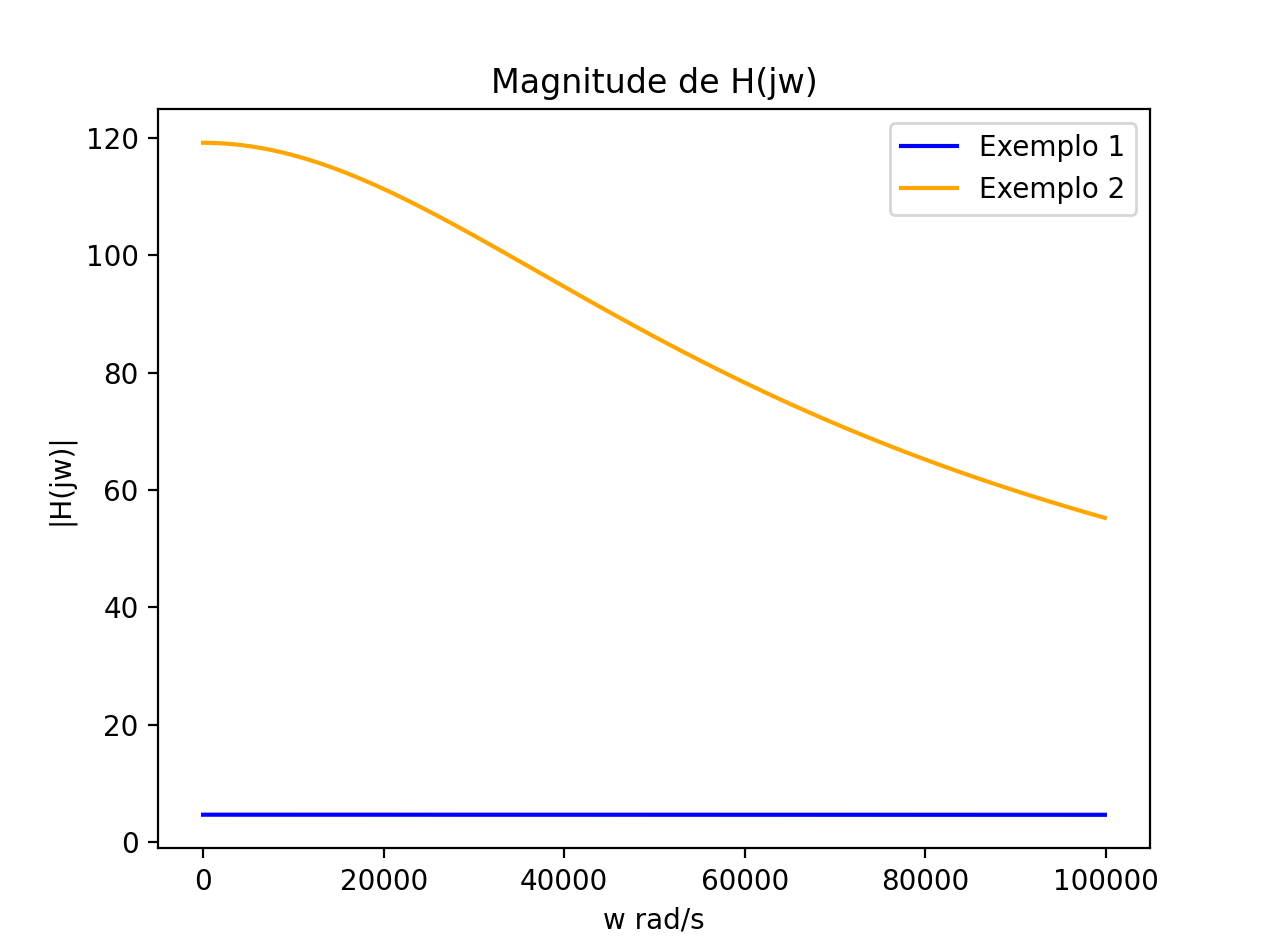
\includegraphics[width=1\columnwidth]{images/plot_bode.png}
    \caption{Gráfico da magnitude pela frequência dos exemplos 1 e 2.}
\end{figure}


\newpage




\section{Medições em laboratório}


Montaremos os dois circuitos discutidos acima em laboratório, e mediremos a tensão de entrada e saída para várias frequências, e com isto obteremos a magnitude da função transferência para frequências diversas.


\begin{figure}[h]
    \centering
    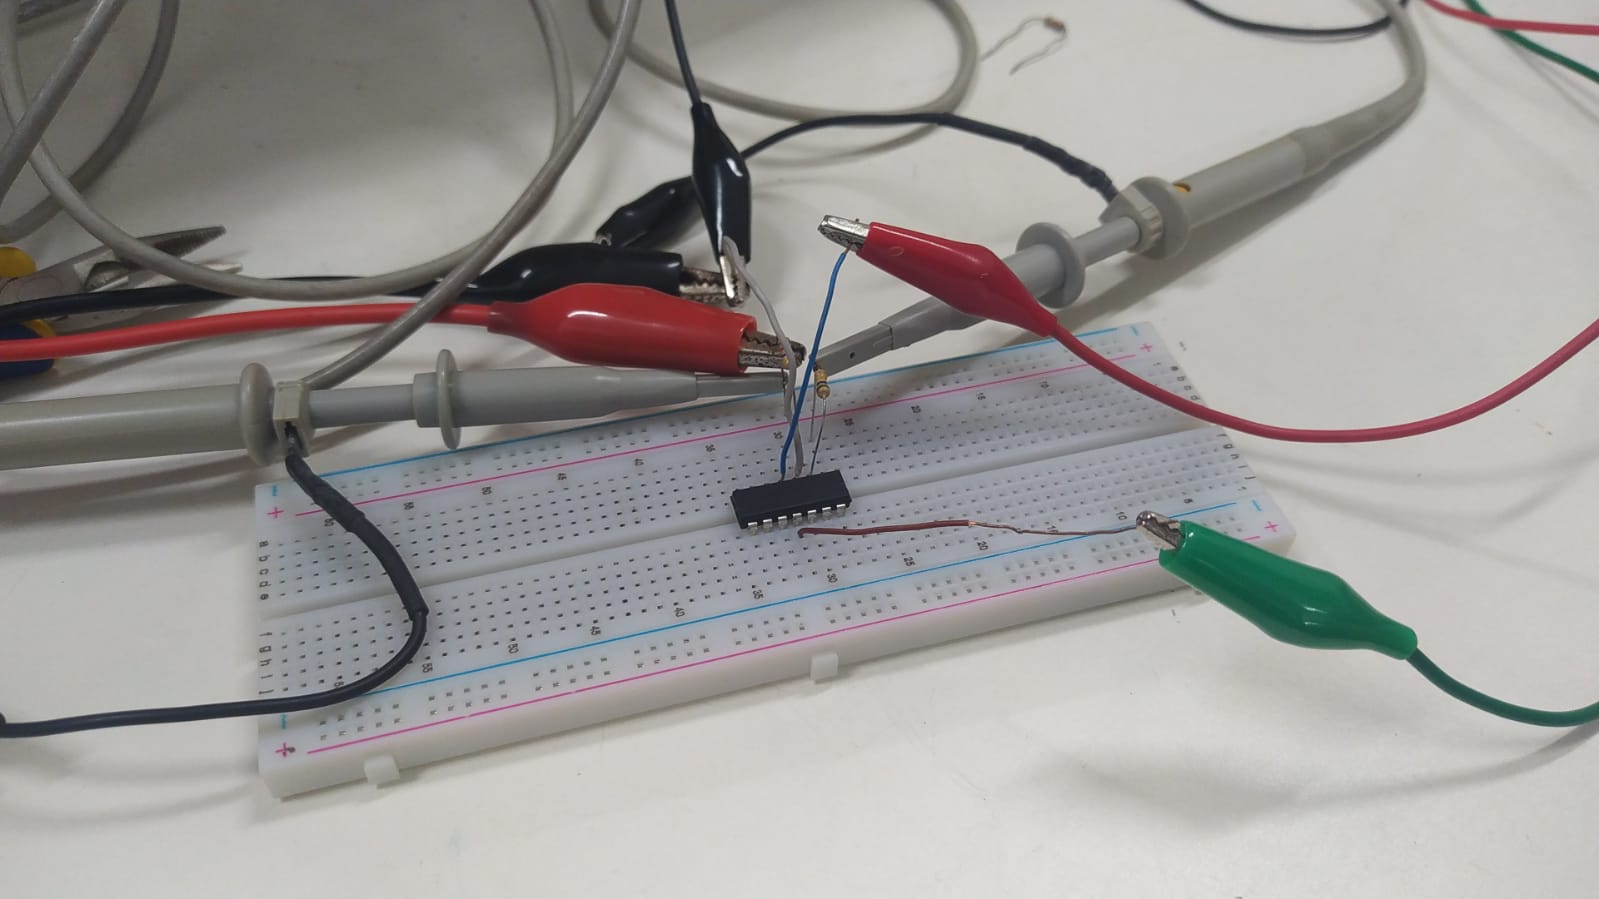
\includegraphics[width=1\columnwidth]{images/circuitoreal.jpeg}
    \caption{Foto do circuito montado em laboratório.}
\end{figure}


\subsection{Circuito 1}


\subsubsection{Valores dos componentes}


\begin{equation}
    \begin{aligned}
        R_1 = 4.65k \varOmega \\
        R_2 = 21.9k \varOmega \\
    \end{aligned}
\end{equation}


\subsubsection{Frequência de corte}


Identificamos a frequência de corte como sendo $f_c = 210 kHz$.


\subsubsection{Valores medidos}


\begin{figure}[H]
    \centering
    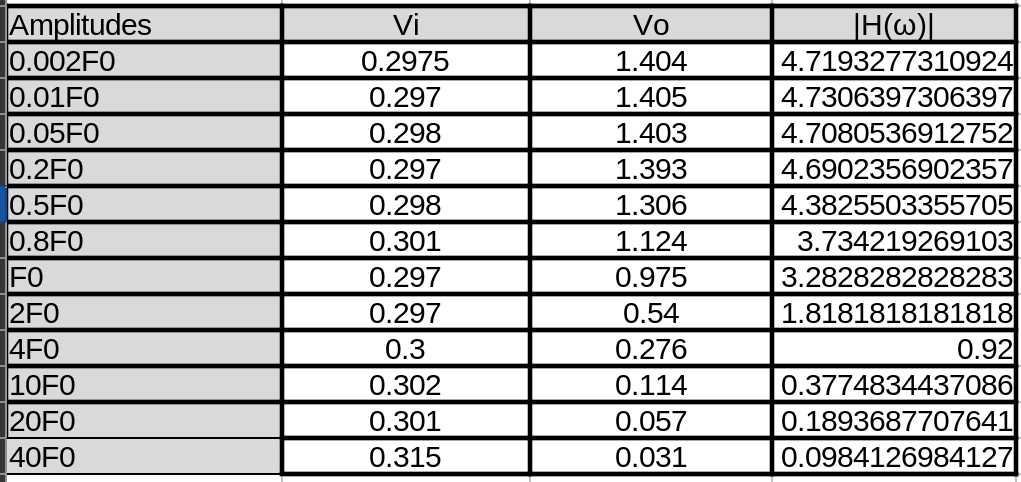
\includegraphics[width=1\columnwidth]{images/valores1.png}
    \caption{Tabela de magnitude para uma gama de valores de frequência.}
\end{figure}


\subsubsection{Fotos do osciloscópio}


\begin{figure}[H]
    \centering
    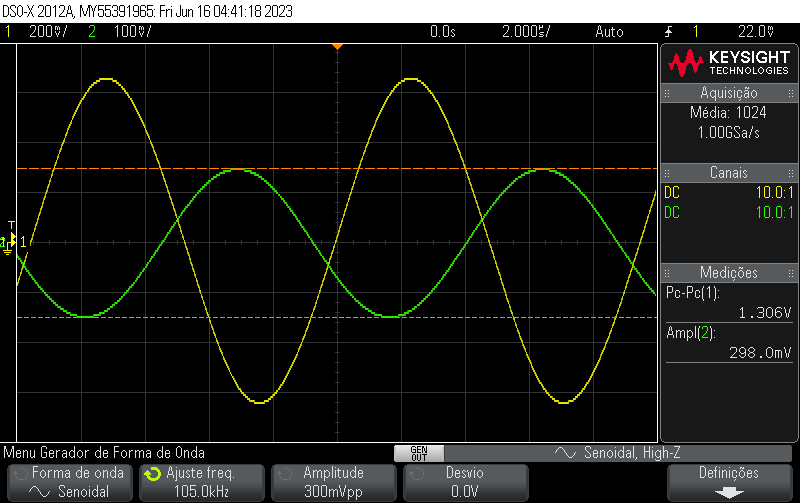
\includegraphics[width=1\columnwidth]{images/exemplo1_meio_fc.png}
    \caption{Imagem da onda no osciloscópio para 0.5 $f_c$.}
\end{figure}


\begin{figure}[H]
    \centering
    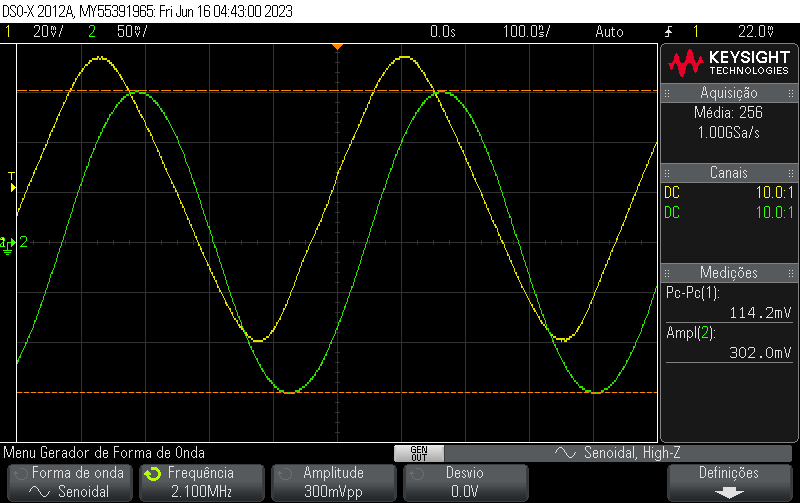
\includegraphics[width=1\columnwidth]{images/exemplo1_10_fc.png}
    \caption{Imagem da onda no osciloscópio para 10 $f_c$.}
\end{figure}


\begin{figure}[H]
    \centering
    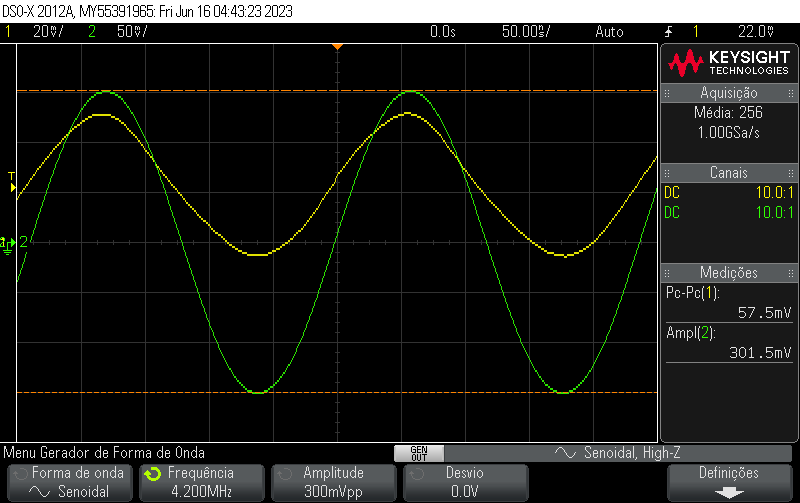
\includegraphics[width=1\columnwidth]{images/exemplo1_20_fc.png}
    \caption{Imagem da onda no osciloscópio para 20 $f_c$.}
\end{figure}
\newpage


\subsection{Circuito 2}


\subsubsection{Valores dos componentes}


\begin{equation}
    \begin{aligned}
        R_1 = 4.65k \varOmega \\
        R_2 = 550k \varOmega  \\
    \end{aligned}
\end{equation}


\subsubsection{Frequência de corte}


Identificamos a frequência de corte como sendo $f_c = 11800 kHz$.


\subsubsection{Valores medidos}


\begin{figure}[h]
    \centering
    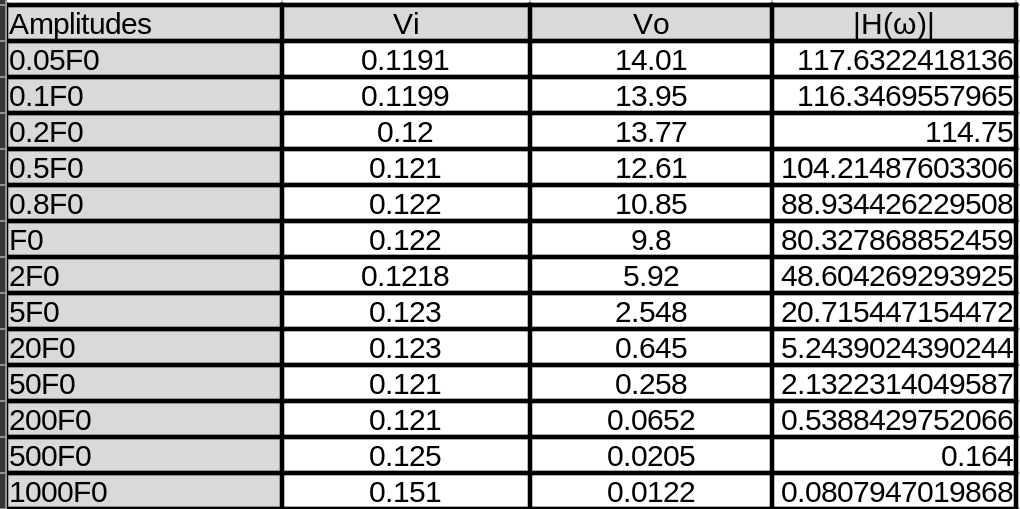
\includegraphics[width=1\columnwidth]{images/valores2.png}
    \caption{Tabela de magnitude para uma gama de valores de frequência.}
\end{figure}


\subsubsection{Fotos do osciloscópio}


\begin{figure}[h]
    \centering
    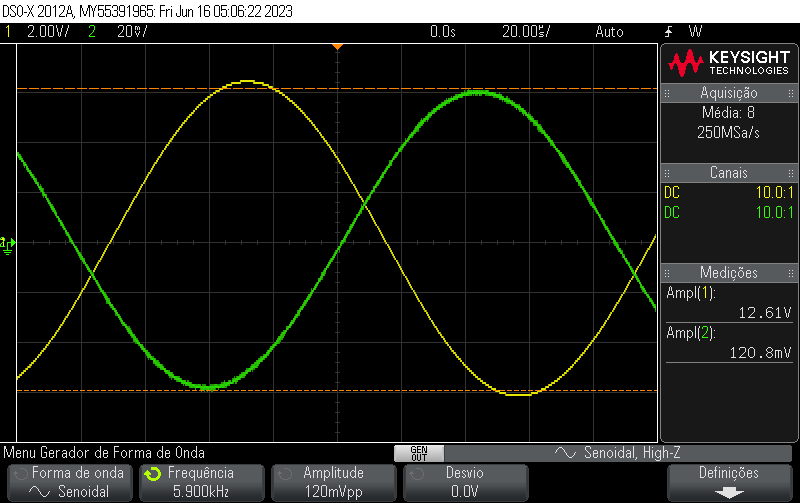
\includegraphics[width=1\columnwidth]{images/exemplo2_meio_fc.png}
    \caption{Imagem da onda no osciloscópio para 0.5 $f_c$.}
\end{figure}


\begin{figure}[h]
    \centering
    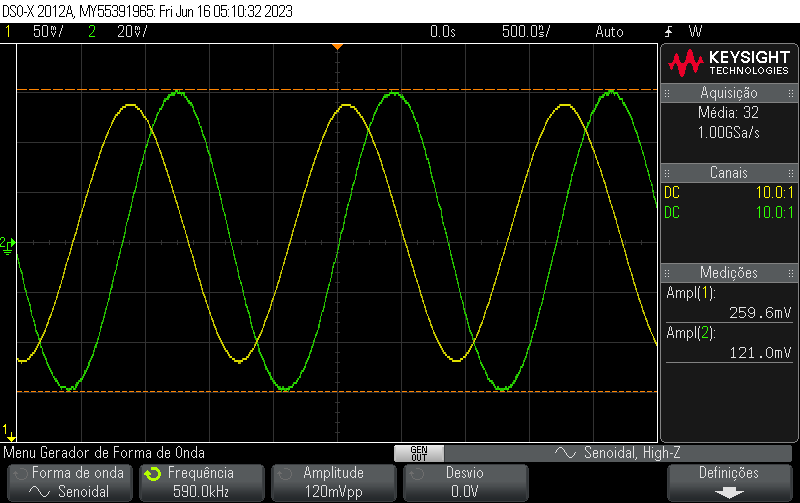
\includegraphics[width=1\columnwidth]{images/exemplo2_50_fc.png}
    \caption{Imagem da onda no osciloscópio para 50 $f_c$.}
\end{figure}


\begin{figure}[h]
    \centering
    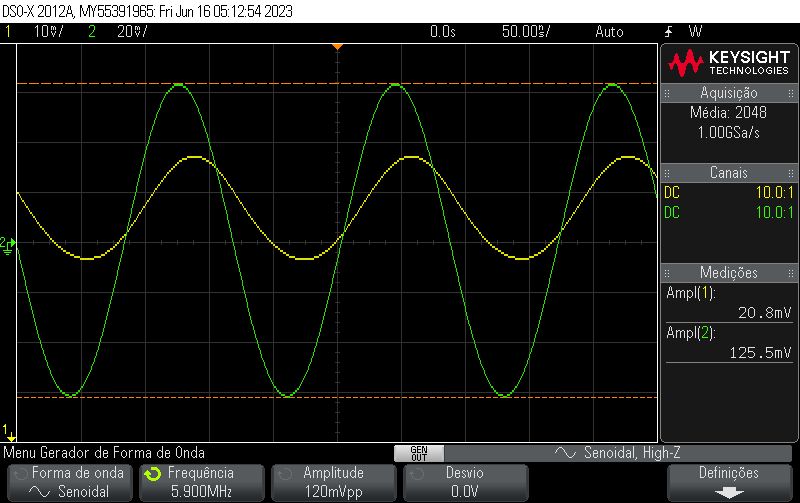
\includegraphics[width=1\columnwidth]{images/exemplo2_500_fc.png}
    \caption{Imagem da onda no osciloscópio para 500 $f_c$.}
\end{figure}


\newpage



\section{Análise dos resultados}


Obtivemos as magnitudes de $H(jw)$ dos exemplos nas figuras (3) e (6), as utilizarei no algoritmo de ajuste de curva que foi disponibilizado no Classroom.


\subsection{Circuito 1}


\subsubsection{Ajuste de curva}


Pelo código de ajuste de curva obtivemos os seguintes valores:


\begin{equation}
    \begin{aligned}
        K   & = -4.9                            \\
        f_c & = 168452.6 Hz = 1.06 * 10^6 rad/s
    \end{aligned}
\end{equation}


Que são coerentes e próximos com os valores achados anteriormente na equação (8).


\subsubsection{Gráfico de Bode}


\begin{figure}[H]
    \centering
    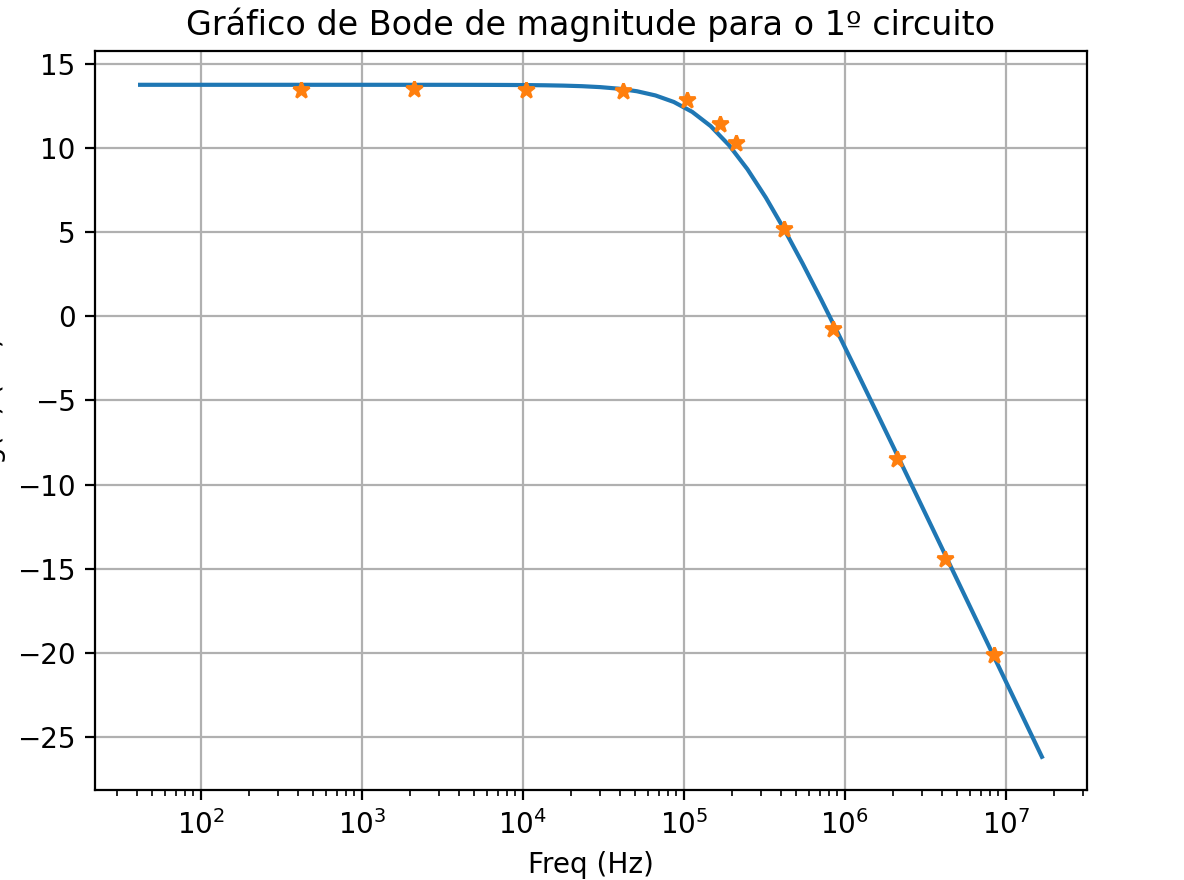
\includegraphics[width=1\columnwidth]{images/bode1.png}
    \caption{Gráfico de Bode para o primeiro circuito.}
\end{figure}

\newpage
\subsection{Circuito 2}


\subsubsection{Ajuste de curva}


Pelo código de ajuste de curva obtivemos os seguintes valores:


\begin{equation}
    \begin{aligned}
        K   & = -120.1                   \\
        f_c & =  9701.2 Hz = 60954 rad/s
    \end{aligned}
\end{equation}


Que são coerentes e próximos com os valores achados anteriormente na equação (9).


\subsubsection{Gráfico de Bode}


\begin{figure}[H]
    \centering
    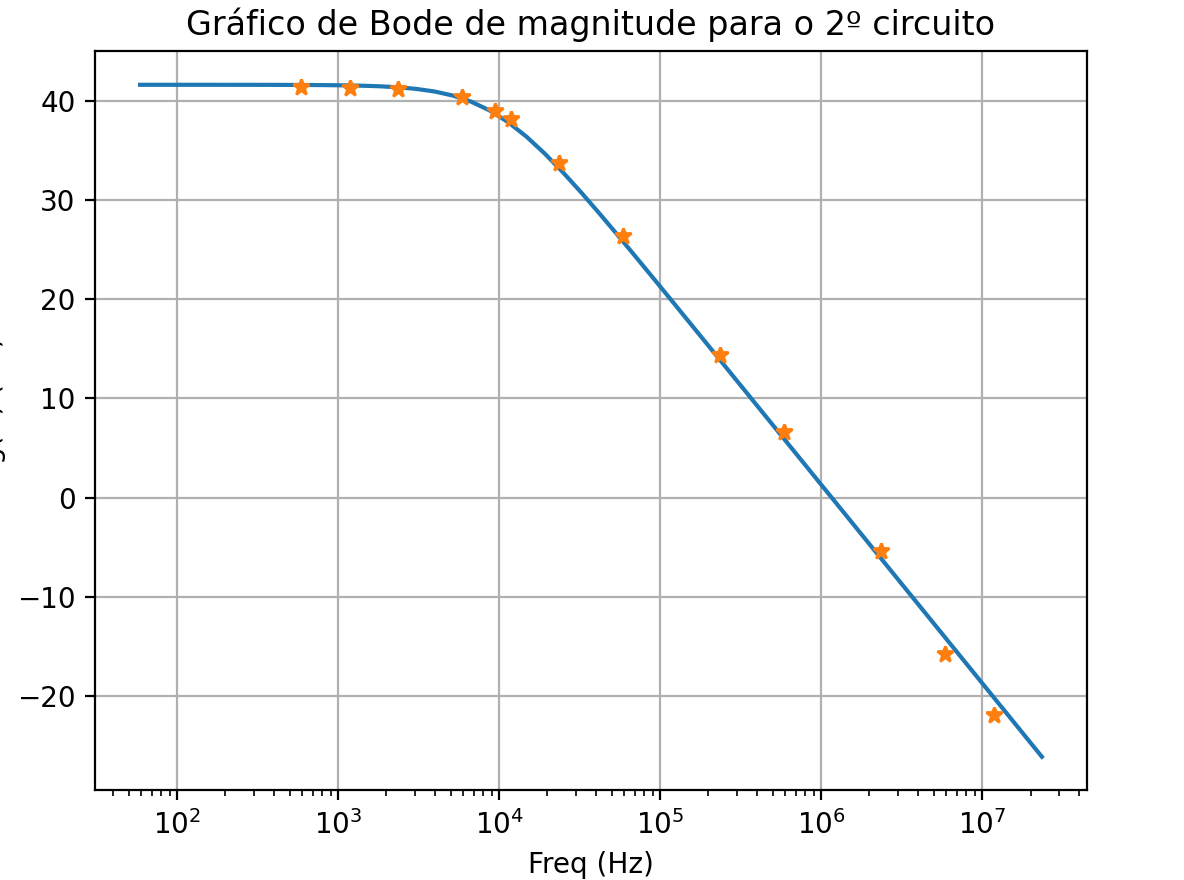
\includegraphics[width=1\columnwidth]{images/bode2.png}
    \caption{Gráfico de Bode para o segundo circuito.}
\end{figure}






\subsection{Gráfico de Bode de ambos circuitos.}


\begin{figure}[H]
    \centering
    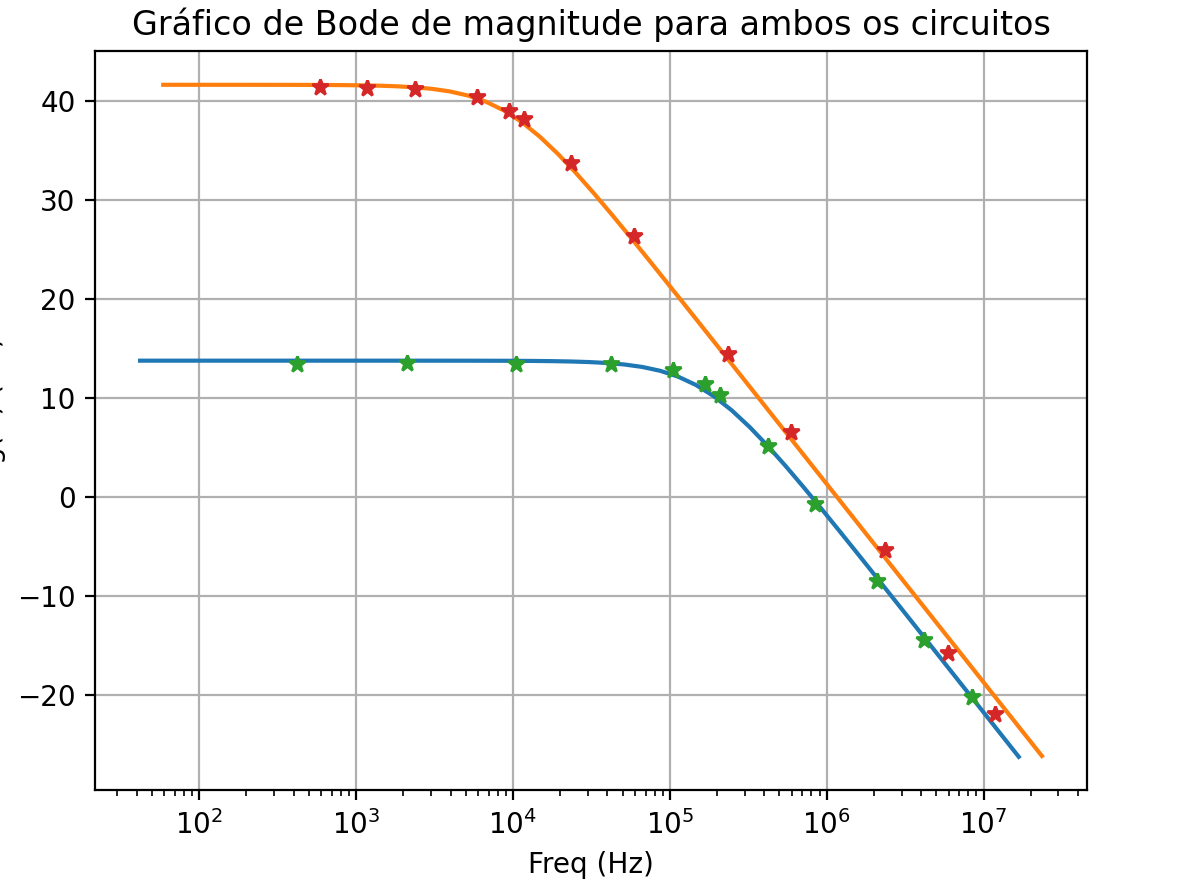
\includegraphics[width=1\columnwidth]{images/bodeboth.png}
    \caption{Gráfico de Bode para ambos circuitos sobrepostos.}
\end{figure}



\section{Conclusões}


Conseguimos com sucesso fazer a análise simbólica e numérica com a biblioteca sympy do Python, e comparamos os resultados com os obtidos experimentalmente.

Nos resultados práticos, obtivemos parâmetros $K$ e $w_c$ bastante similares aos obtidos numericamente.

Observamos que ambos circuitos se comportam como filtros passa-baixa inversores de primeira ordem, que era esperado devido a forma da equação que encontramos na análise preliminar.

Em suma creio que tivemos sucesso em nos familiarizar com as ferramentas de análise de circuitos eletrônicos, e métodos para análise numérica e simbólica.

\section{Apêndice}

Abaixo se encontra o código utilizado para a análise simbólica e numérica do circuito.

\begin{python}
    import matplotlib.pyplot as plt
    import sympy as smp
    from sympy import *

    # Definindo as variaveis simbolicas
    Vo, Vi, Va, Vc, R1, R2, Rp, Cp, A, w, j, Hjw, wp, wc, K = smp.symbols(
    'V_o V_i V_a V_c R_1 R_2 R_p C_p A w j H_jw w_p, w_c, K', real=True)

    # Analise nodal do circuito

    eq1 = smp.Eq((Va - Vi)/R1 + (Va - Vo)/R2 + Va/(Rp + (1/(j * w * Cp))), 0)
    eq2 = smp.Eq(Va * ((1/(j * w * Cp)))/(((1/(j * w * Cp))) + Rp), -Vc)
    eq3 = smp.Eq(A * Vc, Vo)
    # print('Equacoes em latex:')
    # smp.pprint(smp.latex(eq1))
    # smp.pprint(smp.latex(eq2))
    # smp.pprint(smp.latex(eq3))
    # print("")

    print("Equacoes do circuito:")
    print("Equacao 1:")
    smp.pprint(eq1)
    print("Equacao 2:")
    smp.pprint(eq2)
    print("Equacao 3:")
    smp.pprint(eq3)
    print("")

    sols = smp.solve([eq1, eq2, eq3], [Va, Vc, Vo])

    print("Solucao para Vo:")
    smp.pprint(sols[Vo])
    # print("")
    # smp.pprint(smp.latex(sols[Vo]))
    print("")

    print("Aqui fazemos a seguinte simplificacao:")
    print("Rp >> R1 , Rp >> R2, e A >> 1")

    Vo = (-A * R2 * Vi)/((Rp*(R1 + R2))*j*w*Cp + A*R1)

    print("Equacao de Vo simplificada:")
    smp.pprint(Vo)
    # smp.pprint(smp.latex(Vo))
    print("")

    eqHjw = smp.Eq(Hjw, Vo/Vi)

    print("Equacao de Hjw:")
    smp.pprint(eqHjw)
    print("")

    print("Resolvendo a equacao Hjw e colocando no formato canonico da um fitro passa baixa (-K wp / (jw + wp)) obtemos o seguinte:")

    eqHjw = smp.Eq(Hjw, -(K * wc) / (I * w + wc))

    Hjw = -(K * wc) / (I * w + wc)

    smp.pprint(eqHjw)

    print("")

    eqwp = smp.Eq(wp, 1/(Rp*Cp))
    smp.pprint(eqwp)

    eqK = smp.Eq(K, R2/R1)
    smp.pprint(eqK)

    eqwc = smp.Eq(wc, (A*wp)/(1 + K))
    smp.pprint(eqwc)

    print("")

    # Hjw = Hjw.subs({K: R2/R1, wc: A*wp/(1+K)})

    print("Valor absoluto de Hjw:")
    Hjw_abs = smp.Abs(Hjw)
    smp.pprint(Hjw_abs)
    # smp.pprint(smp.latex(Hjw_abs))
    print("")


    print("Exemplo 1:")
    print("Para R1 = 4.7E3 ohms, R2 = 2.2E4 ohms, wp = 2E1 pi e A = 1E5\n")

    eqK1 = eqK.subs({R1: 4.7E3, R2: 2.2E4})
    K1 = smp.solve(eqK1, K)[0]
    smp.pprint(eqK1)
    print("")

    eqwc1 = eqwc.subs({A: 1E5, wp: 20 * smp.pi, K: K1}).evalf()
    wc1 = smp.solve(eqwc1, wc)[0]
    smp.pprint(eqwc1)
    print("")

    print("Valores absolutos para w = [0.5, 1, 2, 4, 10, 20, 40]*wc:")

    # ex1interval = [0.02, 0.01, 0.05, 0.2, 0.5, 1, 2, 4, 10, 20, 40]
    ex1interval = [0.5, 1, 2, 4, 10, 20, 40]

    ex1Vals = []

    for val in ex1interval:
    temp = Hjw_abs.subs({w: wc1 * val, wc: wc1, K: K1})
    ex1Vals.append(temp)
    print('para freq:', round(((val*wc1)/(2*smp.pi)).evalf(), 2),
    '\ttemos:', round(temp, 2))

    print("")

    print("Exemplo 2:")
    print("Para R1 = 4.7E3 ohms, R2 = 5.6E5 ohms, wp = 2E1 pi e A = 1E5\n")

    eqK2 = eqK.subs({R1: 4.7E3, R2: 5.6E5})
    K2 = smp.solve(eqK2, K)[0]
    smp.pprint(eqK2)
    print("")

    eqwc2 = eqwc.subs({A: 1E5, wp: 20 * smp.pi, K: K2}).evalf()
    wc2 = smp.solve(eqwc2, wc)[0]
    smp.pprint(eqwc2)
    print("")

    ex2interval = [0.5, 1, 5, 20, 50, 200, 500, 1000]
    ex2Vals = []

    for val in ex2interval:
    temp = Hjw_abs.subs({w: wc2 * val, wc: wc2, K: K2})
    ex2Vals.append(temp)
    print('para freq:', round(((val*wc2)/(2*smp.pi)).evalf(), 2),
    '\ttemos:', round(temp, 2))
    print("")


    # Plotando os graficos

    frequencias_plot = [i for i in range(1, 100000, 100)]

    plotH1 = [Hjw_abs.subs({w: i, wc: wc1, K: K1}) for i in frequencias_plot]
    plotH2 = [Hjw_abs.subs({w: i, wc: wc2, K: K2}) for i in frequencias_plot]

    fig, ax = plt.subplots()

    ax.plot(frequencias_plot, plotH1, color='blue', label='Exemplo 1')
    ax.plot(frequencias_plot, plotH2, color='orange', label='Exemplo 2')
    ax.legend(['Exemplo 1', 'Exemplo 2'])
    plt.xlabel('w rad/s')
    plt.ylabel('|H(jw)|')
    plt.title('Magnitude de H(jw)')


    plt.show()

    # Medicoes na pratica

    # Exemplo1

\end{python}

\section{Anexos}

Código utilizado para geração de gráficos de bode, e análise utilizando as frequências de cortes obtidas experimentalmente.

\begin{python}
    import numpy as np
    import matplotlib.pyplot as plt
    from scipy.optimize import curve_fit



    fc1 = 210000
    fc2 = 11800


    freqs1 = np.array([0.002*fc1, 0.01*fc1, 0.05*fc1, 0.2*fc1, 0.5*fc1,
            0.8*fc1, fc1, 2*fc1, 4*fc1, 10*fc1, 20*fc1, 40*fc1])
    vin1 = np.array([0.2975, 0.297, 0.298, 0.297, 0.298,
            0.301, 0.297, 0.297, 0.3, 0.302, 0.301, 0.315])
    vout1 = np.array([1.404, 1.405, 1.403, 1.393, 1.306, 1.124,
            0.975, 0.54, 0.276, 0.114, 0.057, 0.031])


    freqs2 = np.array([0.05*fc2, 0.1*fc2, 0.2*fc2, 0.5*fc2, 0.8*fc2, fc2,
            2*fc2, 5*fc2, 20*fc2, 50*fc2, 200*fc2, 500*fc2, 1000*fc2])
    vin2 = np.array([0.1191, 0.1199, 0.12, 0.121, 0.122, 0.122,
            0.1218, 0.123, 0.123, 0.121, 0.121, 0.125, 0.151])
    vout2 = np.array([14.01, 13.95, 13.77, 12.61, 10.85, 9.8, 5.92,
            2.548, 0.645, 0.258, 0.0652, 0.0205, 0.0122])




    def mag_sqr_fun(f, K, fc):
    return (K*fc)**2/(f**2 + fc**2)


    def dB(m):
    return 20*np.log10(m)




    (K1, fc1), _ = curve_fit(lambda f, K, fc: dB(mag_sqr_fun(f, K, fc)),
    freqs1, 2*dB(vout1/vin1))


    print(f"""O ganho K eh {round(K1, 1)}
    A frequencia de corte eh {round(fc1, 1)} Hz""")

    f1 = np.logspace(np.log10(freqs1[0]) - 1, np.log10(freqs1[-1]) + 0.3)
    mag1 = dB(mag_sqr_fun(f1, K1, fc1))/2

    plt.semilogx(f1, mag1)
    plt.semilogx(freqs1, dB(vout1/vin1), "*")
    plt.xlabel("Freq (Hz)")
    plt.ylabel("Mag(H) (dB)")
    plt.title("Grafico de Bode de magnitude para o 1 circuito")
    plt.grid()
    plt.savefig("figura1.png")
    plt.show()



    (K2, fc2), _ = curve_fit(lambda f, K, fc: dB(mag_sqr_fun(f, K, fc)),
    freqs2, 2*dB(vout2/vin2))

    print("\n\nResultados para o 2 circuito:\n")
    print(f"""O ganho K eh {round(K2, 1)}
    A frequencia de corte eh {round(fc2, 1)} Hz""")

    f2 = np.logspace(np.log10(freqs2[0]) - 1, np.log10(freqs2[-1]) + 0.3)
    mag2 = dB(mag_sqr_fun(f2, K2, fc2))/2

    plt.semilogx(f2, mag2)
    plt.semilogx(freqs2, dB(vout2/vin2), "*")
    plt.xlabel("Freq (Hz)")
    plt.ylabel("Mag(H) (dB)")
    plt.title("Grafico de Bode de magnitude para o 2 circuito")
    plt.grid()
    plt.savefig("figura2.png")
    plt.show()




    plt.semilogx(f1, mag1)
    plt.semilogx(f2, mag2)
    plt.semilogx(freqs1, dB(vout1/vin1), "*")
    plt.semilogx(freqs2, dB(vout2/vin2), "*")
    plt.xlabel("Freq (Hz)")
    plt.ylabel("Mag(H) (dB)")
    plt.title("Grafico de Bode de magnitude para ambos os circuitos")
    plt.grid()
    plt.savefig("figura3.png")
    plt.show()

\end{python}


\end{document}